\documentclass[spanish, fleqn]{article}
\usepackage[top=2.5cm, bottom=2.5cm, left=2.5cm, right=2.5cm]{geometry}
\usepackage{babel}
\usepackage[utf8]{inputenc}
\usepackage{fourier}
\usepackage{amsmath, amsfonts, amsthm, fourier}
\usepackage[colorlinks, urlcolor=blue]{hyperref}
\usepackage{xcolor}
\usepackage{listings}
\usepackage{float}
\usepackage{placeins}
\usepackage[T1]{fontenc}
\usepackage{graphicx}
\usepackage{cleveref}[2012/02/15]

\crefformat{footnote}{#2\footnotemark[#1]#3}

\lstdefinestyle{ListingsStyle}{
    language=Python,
    basicstyle=\ttfamily,
    frame=top,frame=bottom,
    commentstyle=\color{red},
    keywordstyle=\color{green!60!black},
    stringstyle=\color{darkgreen},
    rulecolor=\color{gray},
    showspaces=false,
    showstringspaces=false,
    showtabs=false,
    captionpos=b
}
\lstset{escapechar=@,style=ListingsStyle}

\setlength{\parindent}{0pt}
\newcommand{\num}{4}
\title{Tarea \num\\
       \large Algoritmos y Complejidad\\[3ex]
       \emph{Slicing through the 90s}}
\author{Sassy Complexes}
\date{}

\begin{document}
\maketitle

\section{Problema}
Bienvenidos a Horstlandia, el país mas desarrollado del mundo, donde todo es perfecto excepto por un solo detalle: sus edificios son muy altos, tapando la vista de gran parte de sus habitantes. Cansado de escuchar protestas de la población, el benévolo presidente de este país ha decidido tomar acciones y ejecutar la solución más adecuada: cortar edificios al mismo tamaño. Cada calle en este país se puede ver como una secuencia de $n$ edificios, los cuales están compuestos por pisos de igual tamaño. La altura $h_i$ del edificio $i$ se define como la cantidad de pisos que posee.\\

Para rebanar los edificios el presidente ha definido la operación \textbf{slice}, la cual consiste en cortar una secuencia de edificios a cierta altura $H$, es decir, todos los pisos por encima de esta altura serán destruidos. Esta operación conlleva un costo igual a la cantidad de pisos (de cada edificio) que han sido destruidos.\\

El presidente considera que un \textbf{buen slice} es aquel que no sobrepasa un costo $k$, es decir, que no se destruyan más de K pisos en cada corte a la secuencia de edificios.\\

Ahora es su tarea calcular la cantidad mínima de ''\textbf{buenos slices}'' que se pueden realizar a un grupo de edificios tal que todos queden \textbf{del mismo tamaño}. Asuma que se entrega la cantidad $n$ de edificios, el costo de un buen slice $K$ y las alturas $h_i$ de los edificios.

\begin{figure}[ht]
    \centering
    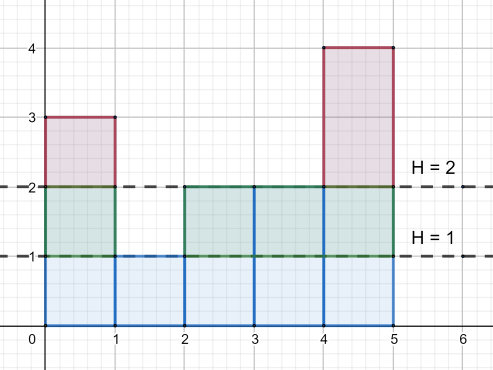
\includegraphics[scale=0.5]{edificios.png}
    \caption{5 edificios. Buen slice no sobrepasa costo 5. Cantidad mínima de buenos slices: 2. Primer corte en $H=2$, costo 3, segundo corte en $H=1$, costo 4.}
    \label{fig:my_label}
\end{figure}

\newpage
\begin{enumerate}
    \item Describa informal (pero claramente) un algoritmo \textbf{voraz} para resolver este problema. Considere que siempre habrá mas de un edificio ($n > 1$) y que el costo máximo de un ''\emph{buen slice}'' es siempre mayor o igual al número de edificios ($k \geq n$). Debe dejar bien claro los pasos y decisiones que realiza su algoritmo\footnote{\label{note1}Explicaciones vagas y chamullos serán castigados severamente.}, puede apoyarse en diagramas y demases que quepan en su informe.
    \item Demuestre formalmente que su algoritmo encuentra el número mínimo de ''\emph{buenos slices}'', es decir un óptimo global\cref{note1}. En caso de suceder, describa las restricciones y acotaciones para las cuales su algoritmo es óptimo, y describa las modificaciones para hacer su algoritmo óptimo para toda posible instancia del problema\cref{note1}.
\end{enumerate}

%\section{Condiciones de Evaluación de código}
Se evaluará:
\begin{itemize}
    \item \textbf{Ejecución correcta}: que funcionen los casos de prueba y \textbf{NO} sea posible encontrar casos en que el programa entregue una respuesta equivocada.
    \item \textbf{Complejidad computacional adecuada}: Que el algoritmo implementado tenga una complejidad igual o mejor que la esperada, y que sea ad-hoc a la materia que se está evaluando (e.g. no utilizar programación dinámica si se pide programar un algoritmo voraz).
    \item \textbf{Calidad del programa}: uso adecuado de funciones, uso de estructuras de control, uso de estructuras de datos, código claro y simple.
    \item \textbf{Código ordenado}: nombres adecuados, indentación correcta, comentarios suficientes, ausencia de código comentado.
\end{itemize}
Para más información refiérase a las condiciones de evaluación del código publicadas en moodle

% Condiciones generales de tareas de Estructuras Discretas, 2015
\section{Condiciones de entrega}

  \begin{itemize}
  \item
    La tarea se realizará \emph{individualmente}
    (esto es grupos de una persona),
    sin excepciones.
  \item
    La entrega debe realizarse vía \href{http://moodle.inf.utfsm.cl}{Moodle}
    en un \emph{tarball} en el área designada al efecto, bajo el formato
    \texttt{tarea-\num-\emph{rol}.tar.gz}
    (\texttt{rol} con dígito verificador y sin guión).
    Puede uzar otra compresión que maneja Moodle,
    como \texttt{xz(1)}.

    Dicho \emph{tarball} debe contener las fuentes en LaTeX
    (al menos \texttt{tarea-\num.tex})
    de la parte escrita de su entrega,
    además de un archivo \texttt{tarea-\num.pdf},
    correspondiente a la compilación de esas fuentes.
  \item
    En  caso de haber programas,
    su ejecutable \emph{debe} llamarse \texttt{tarea-\num},
    de haber varias preguntas solicitando programas,
    estos deben llamarse \texttt{tarea-\num-1},
    \texttt{tarea-\num-2},
    etc.
    Si hay programas compilados,
    incluya una \texttt{Makefile}
    que efectúe las compilaciones correspondientes.

    Los programas se evalúan según que tan claros
    (bien escritos)
    son,
    si se compilan y ejecutan sin errores o advertencias según corresponda.
    Parte del puntaje es por ejecución correcta con casos de prueba.
    Si el programa no se ciñe a los requerimientos de entrada y salida,
    la nota respectiva es cero.
  \item
    Además de esto,
    la parte escrita de la tarea debe en hojas de tamaño carta
    en Secretaría Docente de Informática (Piso 1, edificio F3).
  \item
    Tanto el \emph{tarball} como la entrega física
    deben realizarse el día indicado
    en \href{http://moodle.inf.utfsm.cl}{Moodle}.
    No entregar la parte escrita en papel
    o no entregar en formato electrónico correcto
    tiene un descuento de 50 puntos.

    Por cada día de atraso se descontarán 20 puntos.
    A partir del tercer día de atraso
    no se reciben más tareas,
    y la nota de la tarea es cero.
  \item
    Nos reservamos el derecho de llamar a interrogación
    sobre algunas de las tareas entregadas.
    En tal caso,
    la nota base
    (antes de descuentos por atraso y otros)
    es la de la interrogación.
    No presentarse a la interrogación sin justificación previa
    significa automáticamente nota cero.
  \end{itemize}


\end{document}
